\section{Moderne Webtechnologien}

Das \emph{World Wide Web Consortium (W3C)} standardisiert Technologien die das Internet betreffen. Das Konsortium besteht aus �ber 300 Mitgliedern\footnote{Stand: August 2012} \ref{w3cmembers}, die �ber die Entstehung neuer Standards beraten und entscheiden. Da die Entstehung und Ver�ffentlichung neuer Standards beim W3C auf Grund der hohen Mitgliederzahl und demokratischen Strukturen oft sehr lange dauert, gr�ndeten Vertreter von Opera, Apple und Mozilla die \emph{Web Hypertext Application Technology Working Group (WHATWG)}. Eine Arbeitsgruppe, deren Mitgliedschaft nur auf Einladung erfolgt und deren endg�ltige Entscheidungen einem Vorsitzenden unterliegen. Erarbeitete Entw�rfe reicht die WHATWG beim W3C als Vorschlag zur Standardisierung ein. Einen Vorschlag der WHATWG nahm das W3C auch als Basis f�r die Spezifizierung von \emph{HTML5}. \ref{aboutw3c} \ref{keith}

\subsection{Der HTML5-Standard}
In der Spezifikation des W3C wird mit ``HTML5'' die Weiterentwicklung der Auszeichnungssprache HTML beschrieben. Die WHATWG dehnt den Begriff etwas weiter aus und versammelt unter dieser Bezeichnung auch einige JavaScript-Schnittstellen, wie etwa f�r das canvas-Element (siehe Kapitel \ref{canvasapi}), das \emph{WebSockets}-Netzwerkprotokoll oder die Nutzung von lokalem Speicher (\emph{WebStorage}). Im Sprachgebrauch wird der Begriff ``HTML5'' oft noch weiter gefasst und beinhaltet diverse weitere Technologien, die im Zuge moderner Web-Applikationen entwickelt wurden. Darunter fallen dann die Grafikbibliothek \emph{WebGL}, die \emph{Geo-Location}-API zur Abfrage des Standorts oder auch der \emph{CSS3}-Standard zur Gestaltung von Webseiten. (siehe Abbildung \ref{specgraphfig})

\begin{figure}[h]
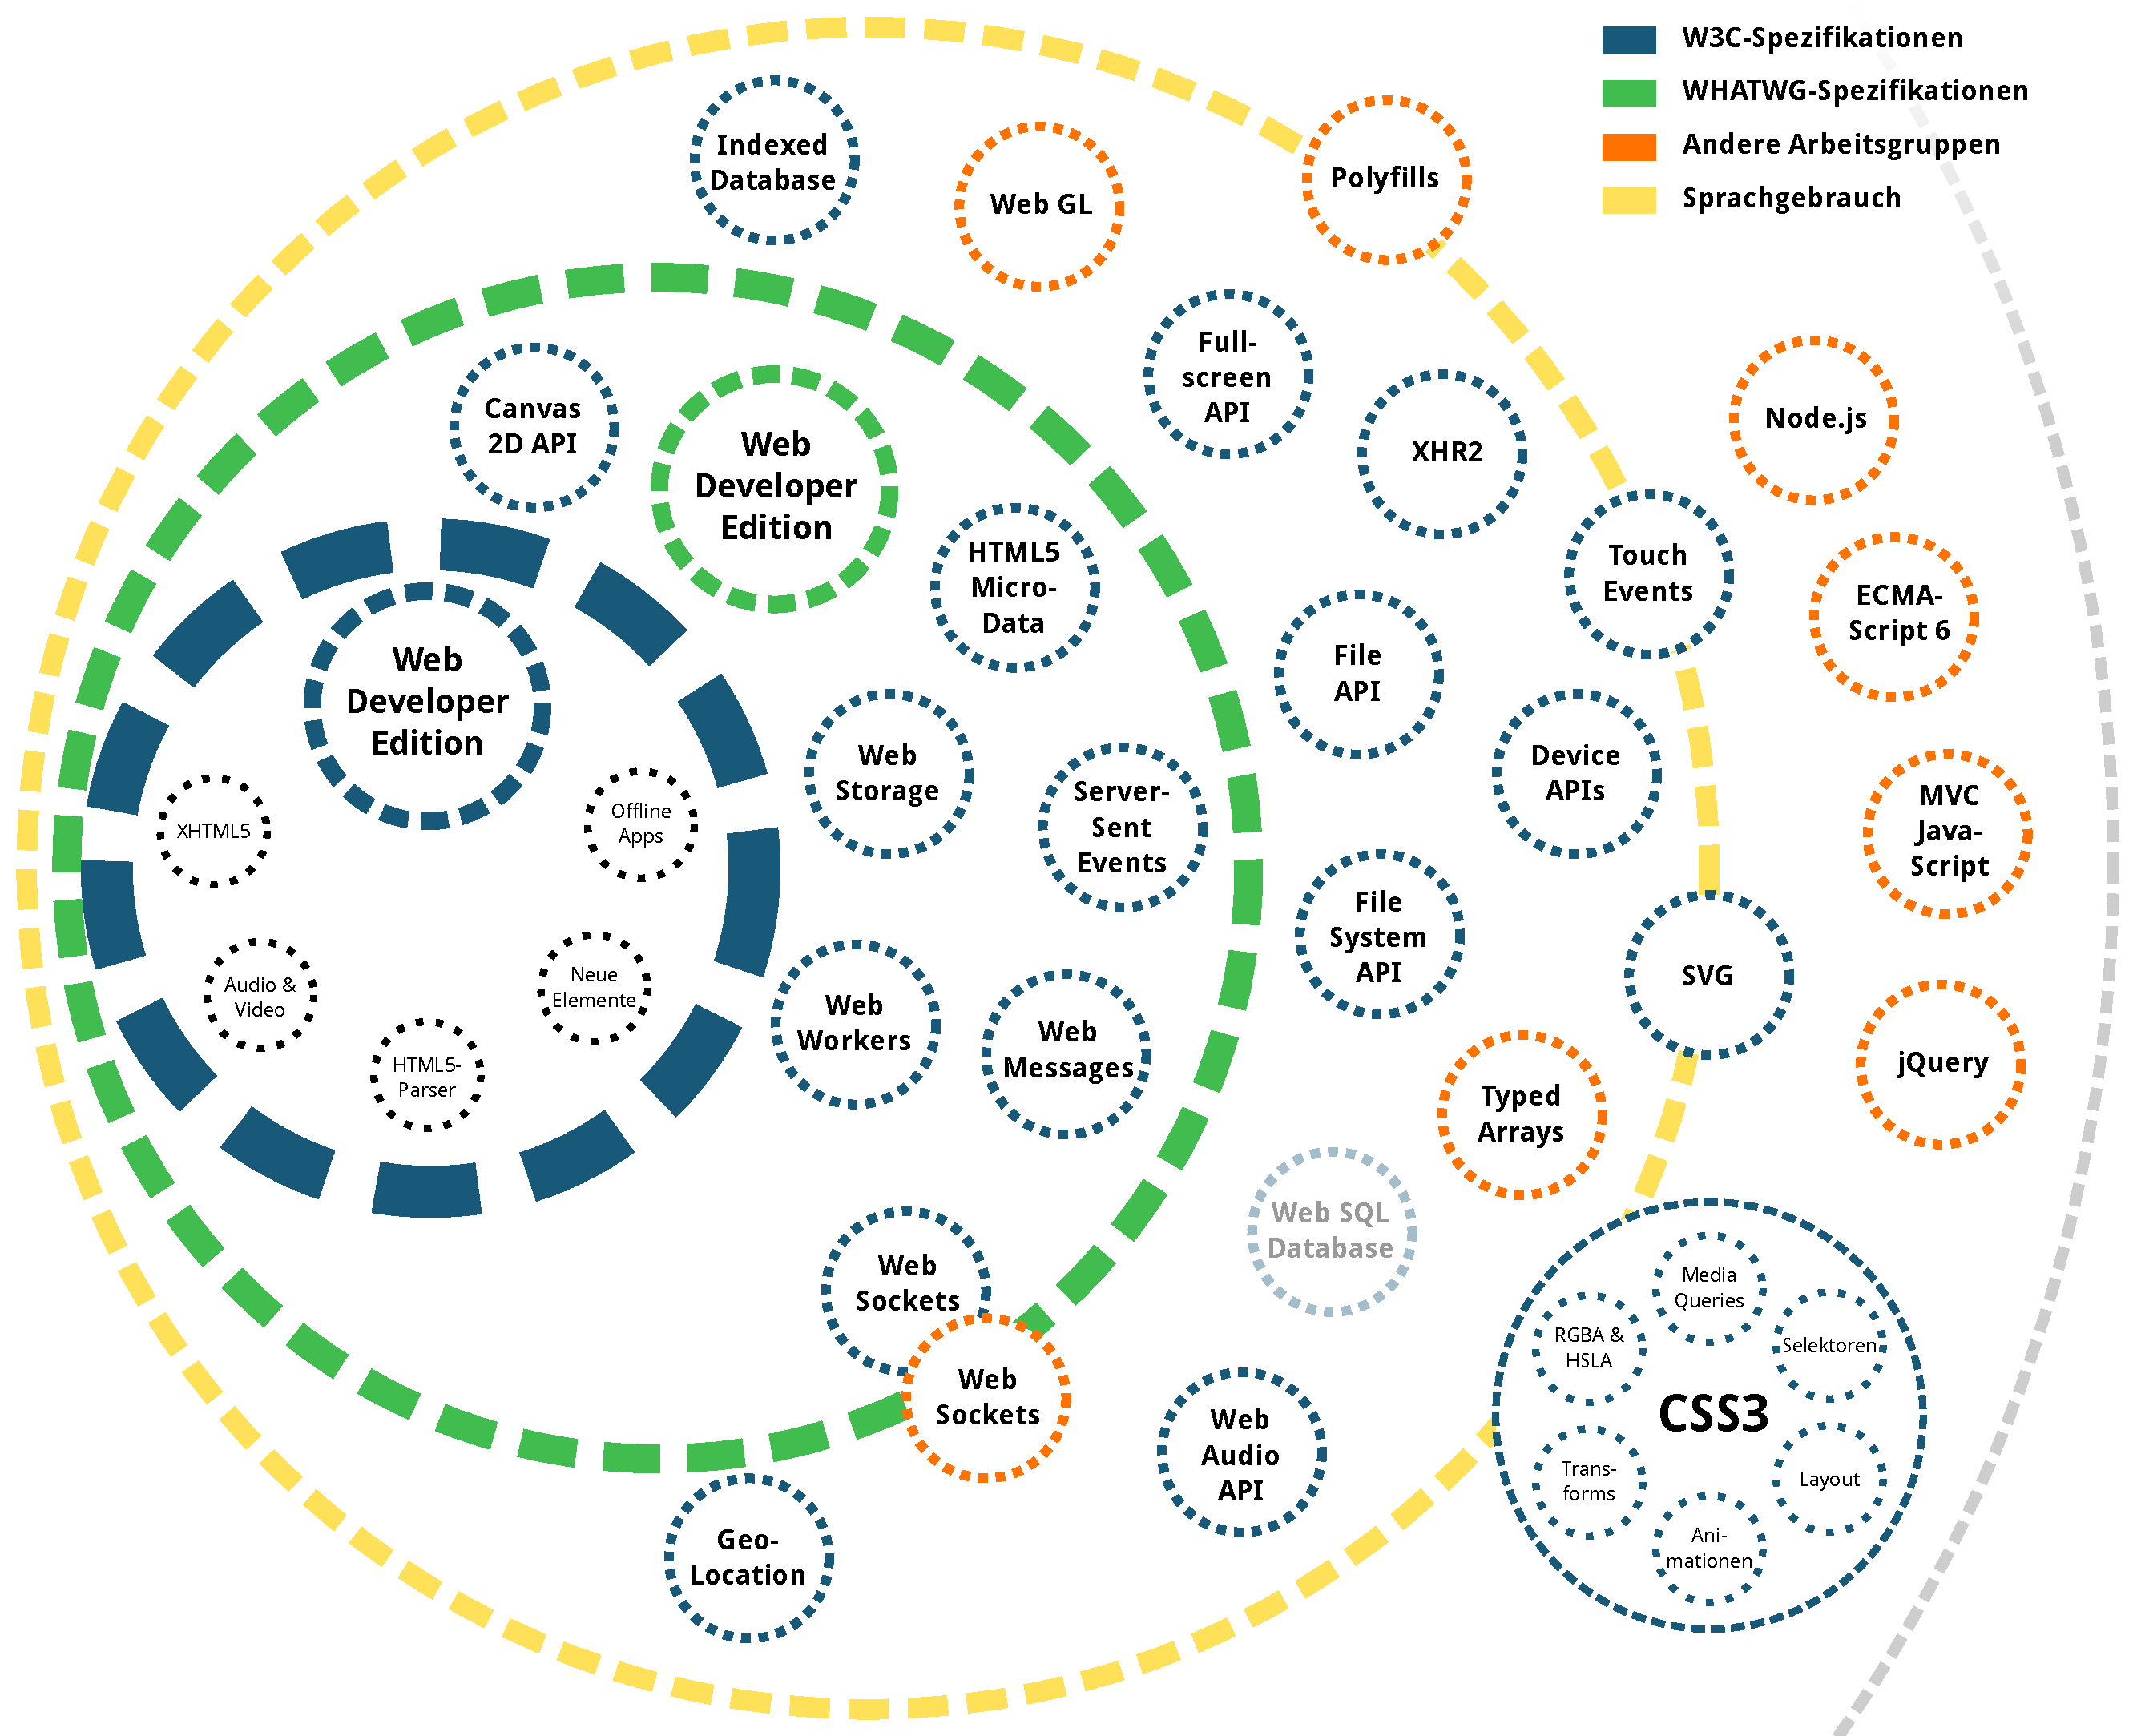
\includegraphics[width=\textwidth]{media/specGraph.pdf}
\caption{HTML5 Spezifikations-�bersicht (CC-BY-3.0 Peter Kr�ner) \cite{specGraph}}
\label{specgraphfig}
\end{figure}



Eine der Design-Entscheidungen bei der Entwicklung von HTML5 ist, den bestehenden Standard HTML 4.01 nicht zu ersetzen, sondern weiterzuentwickeln. Dadurch entsprechen die meisten Webseiten im HTML-4.01-Standard nach Anpassung der Dokumententypdeklaration direkt dem HTML5-Standard. \ref{diveInto}

Die Spezifikation hat den Status ``Last Call''\footnote{Stand: 22. August 2012}. Damit fordert das W3C auf letzte �nderungsvorschl�ge einzureichen, bevor der Standard im Jahr 2014 den Status ``Recommendation'' erhalten soll und damit final ist. Da jedoch die Implementierung in den einzelnen Browsern weit fortgeschritten ist und kaum noch �nderungen am Standard erwartet werden, kann er bereits jetzt eingesetzt werden. \cite{w3cpr}


\subsubsection{DOM und JavaScript APIs}

Nach dem parsen bildet der Browser intern die hierarchische Struktur eines HTML-Dokuments in Form eines Baumes ab. Diese Abbildung wird als \emph{Document Object Model (DOM)} bezeichnet. Der Zugriff auf den DOM-Baum ist mittels einer Schnittstelle (\emph{Application Programmable Interface (API)}) f�r JavaScript-Anwendungen m�glich. Elemente, Attribute und Texte sind als Knoten-Objekte angelegt und k�nnen ausgelesen oder manipuliert werden. \ref{mozdom}

Mit der zunehmenden Nutzung von Web-Applikationen sind auch die Anforderungen an die Browser gestiegen. Zur besseren Interaktion des Nutzers mit dem Browser wurden im Umfeld des HTML5-Standards viele weitere JavaScript-APIs definiert und vom W3C standardisiert (vgl. Abbildung \ref{specgraphfig}). \ref{keith} \ref{diveInto}



\subsubsection{Das canvas-Element}
\label{canvasapi}
Das \emph{canvas}-Element, wie in HTML5 definiert, ist ein rechteckiges Blockelement, das ohne weitere Anweisungen komplett unsichtbar ist: Es hat keinen sichtbaren Rahmen und der Inhalt des Elements ist transparent. In einem Dokument k�nnen sich beliebig viele canvas-Elemente befinden, die komplett unabh�ngig von einander sind. Jedes canvas ist im DOM-Baum verankert und kann mit einer ID versehen werden. Innerhalb des canvas-Elements kann alternativer Inhalt angegeben werden, der angezeigt wird wenn der Browser die Darstellung von canvas-Elementen nicht unterst�tzt. Eine beispielhafte Nutzung des Elements kann wie folgt aussehen: \ref{keith} \ref{diveInto}
\begin{verbatim}
    <canvas id="c" width="300" height="200">Fallback</canvas>
\end{verbatim}
Das Element definiert ein aufl�sungsabh�ngiges Bitmap, das in Echtzeit mit Grafikinhalten gef�llt werden kann. Laut Spezifikation definiert canvas einen JavaScript-Funktionsaufruf \verb+canvas.getContext(contextId [, ... ])+ bei dem ein Schl�sselwort in Form eines Strings als \verb+contextId+ �bergeben wird. \cite{W3Ccanvas} Die \emph{WHATWG} spezifiziert zwei m�gliche Kontexte: \verb+2d+ und \verb+webgl+. \cite{WHATWGcanvasContext} Der Funktionsaufruf liefert ein Objekt zur�ck das die jeweilige API bereitstellt oder \verb+null+ falls ein entsprechender Kontext nicht unterst�tzt wird.

Mittels der 2D-API k�nnen einfache Zeichenoperationen ausgef�hrt werden. Dazu geh�ren Linien, Pfade, Rechtecke, Ellipsen, aber auch Texte oder Bilder k�nnen eingef�gt werden. All diese Operationen werden direkt in der CPU berechnet und sind somit nicht hardwarebeschleunigt. Animationen k�nnen durch st�ndiges Neuzeichnen mittels JavaScript-Timer-Funktionen realisiert werden. \ref{WHATWGcanvas} \ref{diveInto}

\label{initwebgl}


% http://www.whatwg.org/specs/web-apps/current-work/multipage/the-canvas-element.html#drawing-text-to-the-canvas
% http://www.peterkroener.de/was-ist-html5-und-was-nicht-und-was-haette-der-kaiser-dazu-gesagt/